\section{Event-driven agent-based SIR model}
\label{sec:sirmodel}
As use case to develop the concepts in this paper, we use the explanatory SIR model \cite{kermack_contribution_1927}. It is a very well studied and understood compartment model from epidemiology, which allows to simulate the dynamics of an infectious disease like influenza, tuberculosis, chicken pox, rubella and measles spreading through a population. 

In this model, people in a population of size $N$ can be in either one of the three states \textit{Susceptible}, \textit{Infected} or \textit{Recovered} at a particular time, where it is assumed that initially there is at least one infected person in the population. People interact \textit{on average} with a given rate of $\beta$ other people per time unit and become infected with a given probability $\gamma$ when interacting with an infected person. When infected, a person recovers \textit{on average} after $\delta$ time units and is then immune to further infections. An interaction between infected persons does not lead to reinfection, thus these interactions are ignored in this model. This definition gives rise to three compartments with the transitions seen in Figure \ref{fig:sir_transitions}.

\begin{figure}
	\centering
	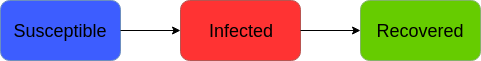
\includegraphics[width=.7\textwidth, angle=0]{./fig1.png}
	\caption{States and transitions in the SIR compartment model.}
	\label{fig:sir_transitions}
\end{figure}

In this paper we follow \cite{macal_agent-based_2010} for translating the informal SIR specification into an event-driven agent-based approach. The dynamics it produces are shown in Figure \ref{fig:sir_sd_dynamics}, which was generated by our own implementation undertaken for this paper, accessible from our repository \cite{thaler_repository_2019}.

\begin{figure}
	\centering
	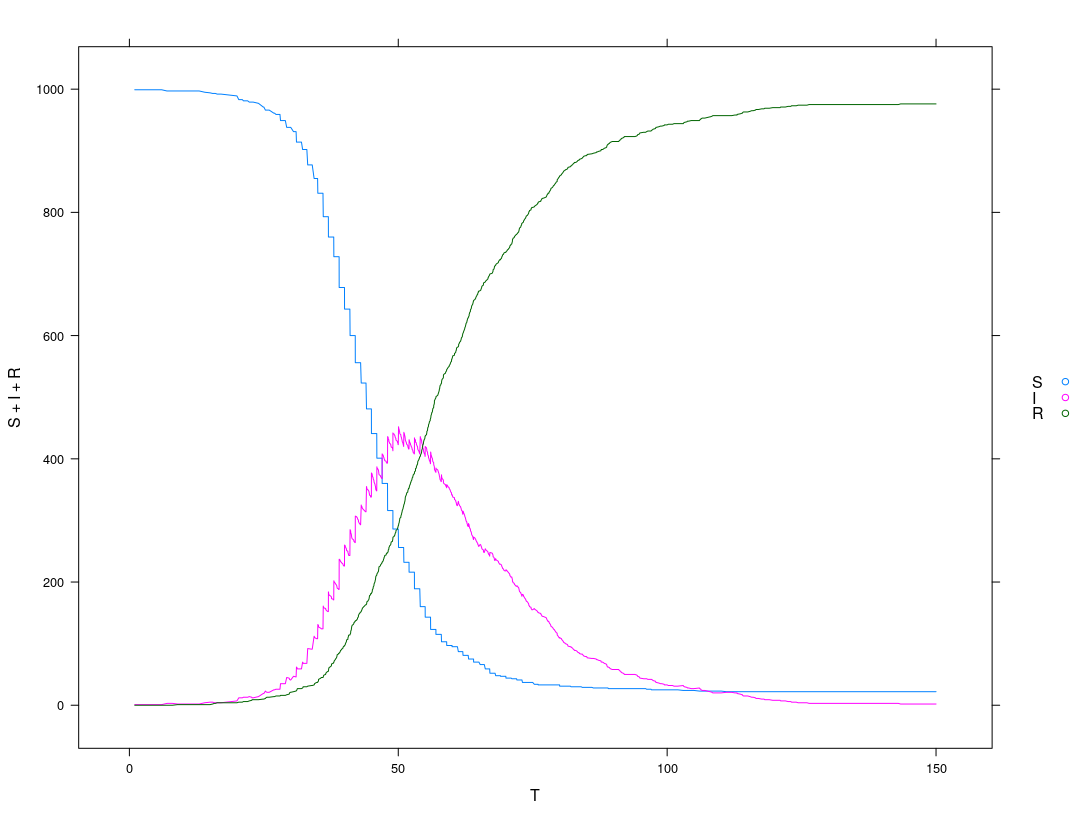
\includegraphics[width=0.7\textwidth, angle=0]{./fig2.png}
	\caption{Dynamics of the SIR compartment model using an event-driven agent-based approach. Population Size $N$ = 1,000, contact rate $\beta =  \frac{1}{5}$, infection probability $\gamma = 0.05$, illness duration $\delta = 15$ with initially 1 infected agent.}
	\label{fig:sir_sd_dynamics}
\end{figure}

\subsection{An informal specification}
In this section we give an informal specification of the agent behaviour, relating the input to according output events. Before we can do that we first need to define the event types of the model, how they related to scheduling and how we can conceptually represent agents.

We are using Haskell as notation and implementation as we conducted our research in that language because it originated property-based testing. We are aware that Haskell is not a mainstream programming language, so to make this paper sufficiently self contained, we introduce concepts step-by-step, which should allow readers, familiar with programming in general, understand the ideas behind what we are doing. Fortunately it is not necessary to go into detail of how agents are implemented as for our approach it is enough to understand the agents' inputs and outputs. For readers interested in the details of how to implement ABS in Haskell, we refer to the work of \cite{thaler_pure_2018}.

We start by defining the states the agents can be in:

%\begin{haskellCode}
\begin{footnotesize}
\begin{verbatim}
-- enumeration of the states the agents can be in
data SIRState = Susceptible | Infected | Recovered
\end{verbatim}
\end{footnotesize}
%\end{haskellCode}

The model uses three types of events. First, \texttt{MakeContact} is used by a susceptible agent to proactively make contact with $\beta$ other agents per time unit by scheduling it to itself. Second, \texttt{Contact} is used by susceptible and infected agents to contact other agents, revealing their id and their state to the receiver. Third, \texttt{Recover} is used by an infected agent to proactively make the transition to recovered after $\delta$ time units.

%\begin{haskellCode}
\begin{footnotesize}
\begin{verbatim}
-- agents are identified by a unique integer
type AgentId = Int
-- enumeration of the three events
data SIREvent = MakeContact | Contact AgentId SIRState | Recover 
\end{verbatim}
\end{footnotesize}
%\end{haskellCode}

As events are scheduled we need a new type to hold them which we termed \texttt{QueueItem} as it is put into the event queue. It contains the event to be scheduled, the id of the receiving agent and the scheduling time.

%\begin{haskellCode}
\begin{footnotesize}
\begin{verbatim}
type Time      = Double
data QueueItem = QueueItem SIREvent AgentId Time
\end{verbatim}
\end{footnotesize}
%\end{haskellCode}

Finally, we define an agent: it is a function, mapping an event to the current state of the agent with a list of scheduled events. This is a simplified view on how agents are actually implemented in Haskell but it suffices for our purpose.

%\begin{haskellCode}
\begin{footnotesize}
\begin{verbatim}
-- an agent maps an incoming event to the agents current state 
-- and a list of scheduled events
sirAgent :: SIREvent -> (SIRState, [QueueItem])
\end{verbatim}
\end{footnotesize}
%\end{haskellCode}

% TODO is there some diagram form (BPNL or other process language, e.g. UML), with which we can express the SIR agents event behaviour? would be more concise than only describing it in word

We are now ready to give the full specification of the susceptible, infected and recovered agent by stating the input-to-output event relations. The susceptible agent is specified as follows:

\begin{enumerate}
	\item \texttt{MakeContact} - If the agent receives this event it will output $\beta$ \texttt{(Contact ai Susceptible)} events, where \texttt{ai} is the agents own id and \texttt{Susceptible} indicating the event comes from a susceptible agent. The events have to be scheduled immediately without delay, thus having the current time as scheduling timestamp. The receivers of the events are uniformly randomly chosen from the agent population. The agent doesn't change its state, stays \texttt{Susceptible} and does not schedule any other events than the ones mentioned.
	
	\item \texttt{(Contact \_ Infected)} - if the agent receives this event there is a chance of uniform probability $\gamma$ that the agent becomes \texttt{Infected}. If this happens, the agent will schedule a \texttt{Recover} event to itself into the future, where the time is drawn randomly from the exponential distribution with $\lambda = \delta$. If the agent does not become infected, it will not change its state, stays \texttt{Susceptible} and does not schedule any events.
	
	\item \texttt{(Contact \_ \_)} or \texttt{Recover} - if the agent receives any of these other events it will not change its state, stays \texttt{Susceptible} and does not schedule any events.
\end{enumerate}

This specification implicitly covers that a susceptible agent can never transition from a \texttt{Susceptible} to a \texttt{Recovered} state within a single event as it can only make the transition to \texttt{Infected} or stay \texttt{Susceptible}. 

The infected agent is specified as follows:

\begin{enumerate}
	\item \texttt{Recover} - if the agent receives this, it will not schedule any events but make the transition to the \texttt{Recovered} state.
	
	\item \texttt{(Contact sender Susceptible)} - if the agent receives this, it will reply immediately with \texttt{(Contact ai Infected)} to \texttt{sender}, where \texttt{ai} is the infected agents' id and the scheduling timestamp is the current time. It will not schedule any events and stays \texttt{Infected}.
	
	\item In case of any other event, the agent will not schedule any events and stays \texttt{Infected}.
\end{enumerate}

This specification implicitly covers that an infected agent never goes back to the \texttt{Susceptible} state as it can only make the transition to \texttt{Recovered} or stay \texttt{Infected}. Also, from the specification of the susceptible agent it becomes clear that a susceptible agent who became infected, will always recover as the transition to \texttt{Infected} includes the scheduling of \texttt{Recovered} to itself. 

\medskip

The \textit{recovered} agent specification is very simple: it stays \texttt{Recovered} forever and does not schedule any events.